\documentclass[11pt]{article}
\usepackage[parfill]{parskip}
\usepackage{graphicx}
\usepackage{wrapfig}
\usepackage{subcaption}
\usepackage[top=1in, bottom=1in, left=1in, right=1in]{geometry}
\bibliographystyle{plain}
\usepackage{amsmath}
\usepackage{amsfonts}
\usepackage{hyperref}
\usepackage[T1]{fontenc}
%%%%%%%%%%%%%%%%%%%%%%%%%%%%%%%%%%%%%%%%%%%%%%%%%%%%%%%%%%%%%%%
\usepackage{fancyhdr}
\pagestyle{fancy}
%%% Please add the author's last names
\lhead{Davis, Theriault, Orhai, Westbrook, and Wright}
\rhead{Modeling the World's Systems, 2019}
%%% Please use \cfoot{} to remove page numbers
\cfoot{ }
\renewcommand{\headrulewidth}{0pt}
\renewcommand{\footrulewidth}{0pt}
%%%%%%%%%%%%%%%%%%%%%%%%%%%%%%%%%%%%%%%%%%%%%%%%%%%%%%%%%%%%%%&
\usepackage{titlesec}
\titlespacing{\section}{0pt}{\parskip}{-.5\parskip}
\titlespacing{\subsection}{0pt}{\parskip}{- .5\parskip}
\titlespacing{\subsubsection}{0pt}{\parskip}{- .5\parskip}
\newcommand{\closeup}{\setlength{\itemsep}{-4pt}}

\newcommand{\amidol}{\textsc{AMIDOL}}

\def\signed #1{{\leavevmode\unskip\nobreak\hfil\penalty50\hskip2em
  \hbox{}\nobreak\hfil(#1)%
  \parfillskip=0pt \finalhyphendemerits=0 \endgraf}}

\newsavebox\mybox
\newenvironment{aquote}[1]
  {\savebox\mybox{#1}\begin{quote}}
  {\signed{\usebox\mybox}\end{quote}}

\date{\vspace{-5ex}}
% Use this to get rid of the date

\usepackage{authblk}
\author{Eric Davis}
\author{Alec Theriault}
\author{Eddy Westbrook}
\author{Ryan Wright}
\affil{Galois, Inc}

%\setcounter{page}{0}



\title{Machine-Assisted Extraction of Formal Semantics from Domain Specific Semi-Formal Diagrams}

\begin{document}
\maketitle
\vspace{10pt}
\begin{abstract}
Analyzing complex systems is a challenging process which requires not only teams of domain experts but often also a multidisciplinary team of data scientists, mathematicians, statisticians, and software engineers in order to support the life cycle of model development, model-based inference, information extraction, and knowledge synthesis.  The models that typically result from this process today are bespoke, lack generalizability, are not performable, lack reusability, and make the task of synthesizing actionable knowledge and policies from their raw outputs difficult.  In this paper we describe \amidol{}: the Agile Metamodel Inference using Domain-specific Ontological Languages, a project that aims to reduce the overhead associated with the development, deployment, maintenance, and reuse of models of complex systems.  Our technique utilizes a common intermediate representation which is designed to support a number of scientific, physical, social, and hybrid domains by allowing domain experts to define their models in a novel way: using domain specific ontological languages (VDSOLs).  The intermediate representation provides formal, executable, meaning to the semi-formal diagrams domain experts normally create, and allows the inference engine to build prognostic queries on associated reward models.  \amidol{} binds results from the inference engine to the original ontologies providing more explainability when compared to conventional methods.
\end{abstract}

\section{Introduction}

The construction of computational models is an important practice for scientists, engineers, policy makers, and other domain experts as it provides a way to make predictions of behavior, to test hypotheses, and to explain witnessed phenomena.  The process of building suitable models, however, is a laborious one which requires diverse teams of experts, significant manual effort, and typical results in models with severe limitations, low performability, and little reusability or generalizability.  Such models are not only costly to produce, both in time and effort, but are also prone to errors, difficult to verify, and do not utilize best practices in software development.

\amidol{} seeks to improve the problems inherent to modern machine-assisted inference with two high-level goals: 1) improving the ability of domain experts to build and maintain models and 2) improving the explainability and agility of the results of machine-inference.  \amidol{} achieves these goals by utilizing a universal intermediate representation which provides executable representations to semantic concepts in a directed graph framework, and translates these representations to traditional machine learning and model solution techniques providing computational meaning to the semi-formal diagrams already being generated by domain experts.

\begin{figure}
  \centering
  \begin{subfigure}[b]{0.48\textwidth}
    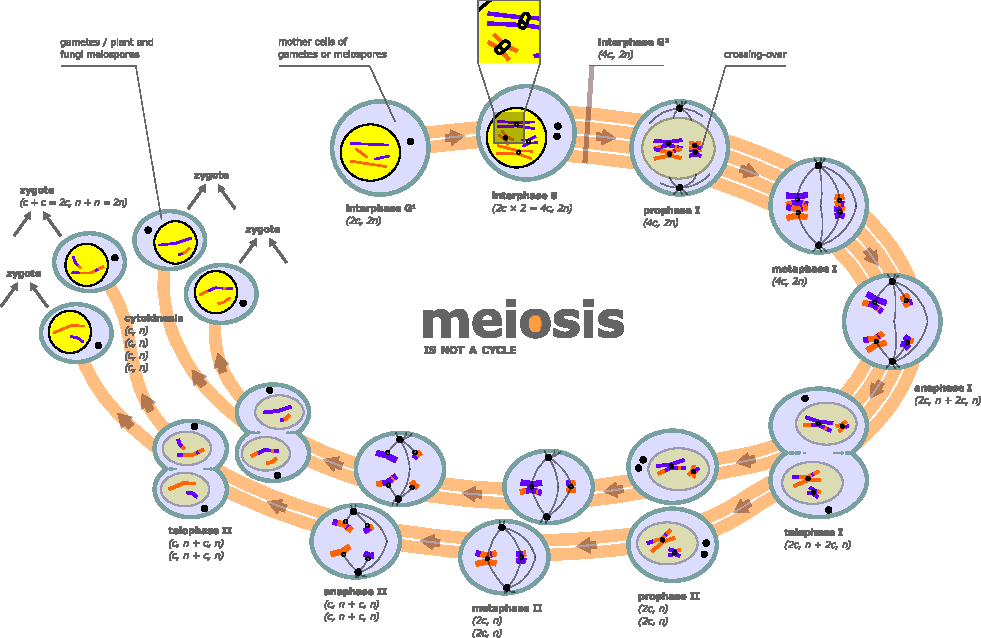
\includegraphics[width=\textwidth]{figs/Diagram_of_meiosis.pdf}
    \caption{Example of a semi-formal diagram of Meoisis. CC-BY-SA 3.0 Marek Kultys, July 2, 2008.}
    \label{Fig:Meiosis}
  \end{subfigure}
  \begin{subfigure}[b]{0.48\textwidth}
    \includegraphics[width=\textwidth]{figs/HIV-Tat-figure.pdf}
    \caption{Example of a semi-formal diagram of the molecular model of the Tat transactivation circuit.}
    \label{Fig:HIV-Tat}
  \end{subfigure}
  \caption{Examples of semi-formal diagrams drawn by domain experts to represent operational semantics and complex
  system models.}
  \label{Fig:Semi-formal}
\end{figure}

Current modeling formalisms are often specified in formal languages which seem arcane and unnatural to domain experts, but have unambiguous formal mathematical meaning.  By contrast domain experts have naturally developed visual semi-formal ways of describing the systems they study, such as those illustrated in Figure \ref{Fig:Semi-formal}, but which are often ambiguous and lack formal mathematical meaning.  In Luca Cardelli's paper on the abstract machines of systems biology \cite{cardelli2005abstract} he notes that these semi-formal diagrams come close to capturing the operational semantics of process algebras, a concept he expanded on when deriving a formal calculus of membrane interactions \cite{cardelli2004brane}.  While Cardelli was able to provide a calculus for a single sub-domain, the need for formal languages which describe biological, physical, or chemistry in an intuitive way was highlighted in Paul Nurse's 2008 paper \cite{nurse2008life}:

\begin{aquote}{Paul Nurse (2008)}
"There should be
a concerted programme \ldots which will require both the development of
the appropriate languages to describe information processing in biological systems and the generation of more effective methods to
translate biochemical descriptions into the
functioning of the logic circuits that underpin
biological phenomena."
\end{aquote}

\paragraph{Significance}
\amidol{} seeks to provide a framework for the development of models which formally describe biological systems and complex systems from other domains using visual domain specific languages backed by a domain inspecific intermediate representation.  This framework provides several significant advancements on the state of the art which seek to improve the usability, maintainability, reusability, and performability of scientific models.  First, \amidol{} will provide translators from many Visual Domain Specific Ontological Languages (VDSOLs) to a single intermediate representation allowing VDSOLs to be specified for new domains and extended easily.  Second, \amidol{} will provide transformations on models in its intermediate representation to optimize the execution of these models, compose models to build more powerful and complex representations, and to overlay reward structures on these models to specify metrics of interest and experiments to perform with \amidol{}'s inference engine.  Finally, \amidol{} provides translations from models in the intermediate representation into solver targets for the inference engine, checking constraints of composed reward structures and solving for measures of interest.  \amidol{} allows these results to be communicated back to the user through the VDSOL, relating raw statistical and machine learning output to the original graph to improve explainability.

\section{AMIDOL}

\begin{figure}
  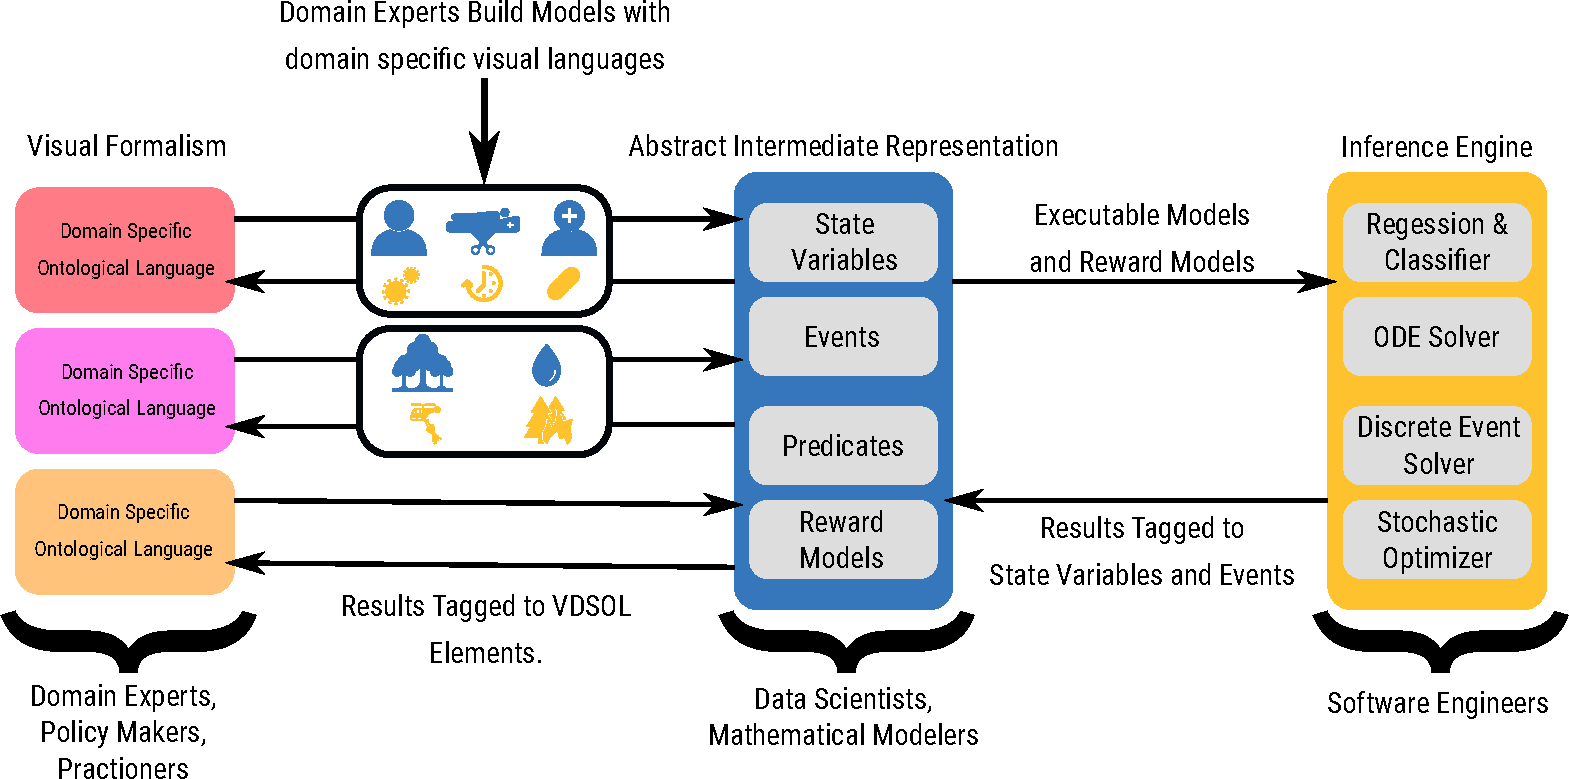
\includegraphics[width=\textwidth]{figs/system-architecture-quad.pdf}
  \caption{\amidol{} Architecture}
  \label{Fig:Architecture}
\end{figure}

Figure \ref{Fig:Architecture} outlines \amidol{}'s architecture and usage pattern. Users define models in one of a number of predefined VDSOLs using directed graphs connecting nouns and verbs.  Each noun or verb has an underlying representation in the intermediate representation.  These representations are then composed together with state sharing \cite{sanders1991reduced}, and then composed with reward models which define metrics of interest.  The resulting composed model can be further transformed in the intermediate representation for performability, efficiency, or other optimizations. \amidol{} then translates the model into a back end solver target, through code or script generation, and associates the results of executing a given solver with a set of nouns or verbs in the VDSOL to provide better explainability.

\paragraph{Visual Domain Specific Languages:}

\amidol{} is designed to support the definition of ontological languages which describe systems as directed graphs of nouns and verbs.  Nouns and verbs for a given domain are organized into \emph{palettes}. Nouns define elements which make up the state space of a system, and verbs define transitions in the state space.  VDSOLs enable domain experts to build models of complex systems which are easier to maintain, validate, and verify, and avoid common pitfalls of monolithic and hand-coded implementations.  To provide visual context for modelers \amidol{} supports the use of arbitrary scalable vector graphics (SVGs) to represent nouns and verbs, and features a canvas on which to draw nouns and verbs.

\paragraph{Composability of Atomic Models:}

\amidol{} is being designed to support the composition of individual models to enable model reuse, compositional methods for solution, to enhance backend support for performance optimizations such as symmetry detection, and to allow domain scientists to experiment by swapping out components of a model which may represent hypotheses about individual elements.  Model composition in \amidol{} is being designed to support two primary mechanisms: \emph{state-sharing} \cite{sanders1992dependability,sanders1988construction} and \emph{event-synchronization} \cite{lampka2002symbolic}.

\paragraph{Intermediate Representation:}

The Intermediate Representation (IR) for \amidol{} is designed to be a universal way to specify models, regardless of their domain, and provides a Turing-complete way to specify models performably, while avoiding domain specific considerations. The IR employed by \amidol{} has its roots in Markov models \cite{howard2012dynamic}, Generalized Stochastic Petri-nets with inhibitor arcs \cite{chiola1993generalized} (which have been shown to be Turing complete), and stochastic activity networks \cite{movaghar1985performability,sanders2000stochastic} (which are extensions of Petri-nets that allow more compact model specification).  \amidol{} currently extends these concepts by creating ways to link to the original VDSOL, and by allowing embedded reward structures to be linked to a graph-based results database which stores the outcomes of experiments and can be used for the construction of arbitrary measures to support inference needs.

Formally, the IR is a 5-tuple, $(S, E, L, \Phi, \Lambda, \Delta)$ where:
\begin{itemize}
\item $S$ is a finite set of state variables $\{s_0, s_1, \ldots, s_{n-1}\}$ that take on values in $\mathbb{N}$.
\item $E$ is a finite set of events $\{e_0, e_1, \ldots, e_{m-1}\}$ that may occur in the model.
\item $L: S|E \rightarrow \mathbb{N}$ is the event and state variable labeling function that maps elements of $S$ and $E$ into the original ontology.
\item $\Phi: E \times N_0 \times N_1 \times \ldots \times N_{n-1} \rightarrow \{0, 1\}$ is the event enabling predicate.
\item $\Lambda: E \times N_0 \times N_1 \times \ldots \times N_{n-1} \rightarrow (0, \infty)$ is the transition rate specification.
\item $\Delta: E \times N_0 \times N_1 \times \ldots \times N_{n-1} \rightarrow N_0 \times N_1 \times \ldots \times N_{n-1}$ is the state variable transition function specification.
\end{itemize}

Informally the IR is used to give formal definition to nouns, verbs, or entire models defined in a given VDSOL. \textbf{state-variables} and their current values make up the state of the model, and measure the configuration and capabilities of all modeled components.  While state variables are defined as taking on values in $\mathbb{N}$, this does not restrict them from representing real numbers to arbitrary precision in modern computer hardware.  In practice, they are implemented as integers, and floating point numbers by \amidol{}.

\textbf{Events}, when fired, change the state of a model by altering the value of state variables.  Events in \amidol{} are associated with \textbf{input predicates} which define the enabling conditions of an event, \textbf{output predicates} which define the side effect of event firing, and a rate function which is used to calculate the inter-firing time of a given event.

An \textbf{input predicate} is associated with an event, and a set of state variables.  Input predicates are functions of the value of their set of variables which map these sets and their values onto the set $\{0, 1\}$.  When an input predicate evaluates to $1$, the event is considered enabled and may fire.  When the input predicate evaluates to $0$, the event is considered disabled and cannot fire until subsequently enabled.  An \textbf{output predicate} is associated with an event, and a set of state variables.  Output predicates map a set of state variables, and their values, to new values for the same state variables defining the side effects of event firing on the state of the model.

\section{Reward Variables, Reward Models, and Inference}

The \amidol{} intermediate representation allows for the specification of reward variables or structures over a given model, and the composition of these structures with a model to produce new models which can be solved by the inference engine.  We define two basic types of rewards structures, rewards over state variable values (rate rewards), and rewards over events (impulse rewards). \cite{qureshi1996algorithms,deavours1999efficient,ciardo1996well,sanders1991reduced}
A rate reward is formally defined as a function $\mathcal{R}: P(S, \mathbb{N}) \rightarrow \mathbb{R}$ where $q \in P(S, \mathbb{N})$ is the reward accumulated when, for each $(s,n) \in q$, the value of the state variable $s$ is $n$.  Informally a rate reward variable $x$ accumulates a defined reward whenever a subset of the state variables take on prescribed values. An impulse reward is formally defined as a function $\mathcal{I}: E \rightarrow \mathbb{R}$ where $e \in E, \mathcal(I)_e$ is the reward for the completion of $e$.  Informally an impulse reward variable $x$ accumulates a defined reward whenever the event $e$ fires.

Both rate and impulse reward variables measure the behavior of a model $M$ with respect to time.  As such, a reward variable $\theta$ is declared as either an instant-of-time variable, an interval-of-time variable, a time-averaged interval-of-time variable, or a steady state variable.  An instant of time variable $\theta_t$ is defined as:

\[ \theta_t = \sum_{\nu \in P(S, \mathbb{N})} \mathcal{R}(\nu) \cdot \mathcal{I}^{\nu}_t + \sum_{e \in E} \mathcal{I}(e) \cdot I_t^e\]

Intuitively a rate reward declared as an instant-of-time variable \cite{freire1990technique} can be used to measure the value of a state variable precisely at time $t$, and an impulse reward declared as an instant-of-time variable can be used to measure whether a given event fired at precisely time $t$.  While the latter is not a particularly useful measure (as the probability of an event with a firing time drawn from a continuous distribution at time $t$ is $0$) it is defined for closure reasons, and for cases with discrete distributions and discrete time steps.

An interval-of-time variable intuitively accumulates reward over some fixed interval of time $[t, t+1]$.  Given such a variable $\theta_{[t, t+1]}$ we formally define interval-of-time variables as:

\[\theta_{[t,t+1]} = \sum_{\nu \in P(S, \mathbb{N})} \mathcal{R}(\nu) \cdot \mathcal{J}^{\nu}_{[t, t+1]} + \sum_{e \in E} \mathcal{I}(e)N^e_{[t,t+1]}\]

where $J^{\nu}_{[t,t+1]}$ is a random variable which represents the total time the model spent in a state such that for each $(s, n) \in \nu$, the state variable $s$ had a value of $n$ during the period $[t, t+1]$. Similarly $I^e_{t\rightarrow\infty}$ is a random variable which represents the number of times an event $e$ fired during the period $[t, t+1]$.

Time-averaged interval of time variables quantify accumulated reward averaged over some interval of time.  Such a variable $\theta'_{[t,t+1]}$ is defined formally as $\theta'_{[t,t+1]} = \frac{\theta_{[t,t+1]}}{l}$.

Steady state reward variables are realized by testing for initial transients, and calculating an instant of time variable after a model has reached a stable steady state with high confidence.

\section{Conclusions}

We are currently testing \amidol{} using the SIS/SIR compartmental model of epidemiology.  While simple, the SIS/SIR model utilizes real data from the CDC, and has a strong set of predictive capabilities.  The primary objective of the SIS/SIR model is to identify the \emph{basic reproduction number} associated with an infection, also known as $R_0$. The importance of estimating $R_0$ has been well established for many historical epidemics, including H1N1 \cite{fraser2009pandemic} and Ebola \cite{fisman2014early}.  This model also lends itself to testing \amidol{}'s Design of Experiments module via public CDC Data on influenza infections by region and year \cite{cdc2019fluview}, episodes which are well modeled by the SIR model.

Our initial tests with \amidol{} suggest that the framework can reduce the reliance of domain experts on bespoke and custom code.  By providing an intermediate representation which is Turing complete, and expressive enough to allow the IR to be transformed to improve performance or tractability, such as when solving stiff systems of ODEs \cite{enright1975comparing} we hope to enable domain experts to leverage the work of software engineers and mathematicians in a repeatable, and reusable way.  By providing a common language for the expression of models and reward structures we hope to improve model maintainability, and to improve the ability of domain experts to share their results, and leverage models created by others in their domain, or even in adjacent domains.  The end goal of \amidol{} is to create a community around this new framework similar to that of LLVM \cite{lattner2004llvm} with an open API for writing transformations for the IR, repositories of VDSOLs and models, and support for various back end solvers enabling more repeatable science utilizing machine-assisted inference.

\section{Acknowledgments}

This research has been supported by DARPA contract DARPA-PA-18-02-AIE-FP-039.

\section{Resources, web sites, etc.}

The current \amidol{} source code, including example models and documentation, is available at the \amidol{} Github site \url{https://github.com/GaloisInc/AMIDOL}.


%\newcommand*{\doi}[1]{\href{http://dx.doi.org/#1}{doi: #1}}
\begin{thebibliography}{10}

\bibitem{cardelli2004brane}
Luca Cardelli.
\newblock Brane calculi.
\newblock In {\em International Conference on Computational Methods in Systems
  Biology}, pages 257--278. Springer, 2004.

\bibitem{cardelli2005abstract}
Luca Cardelli.
\newblock Abstract machines of systems biology.
\newblock In {\em Transactions on Computational Systems Biology III}, pages
  145--168. Springer, 2005.

\bibitem{cdc2019fluview}
CDC.
\newblock National, regional, and state level outpatient illness and viral
  surveillance.
\newblock https://www.cdc.gov/flu/weekly/fluactivitysurv.htm.
\newblock Accessed: January 2019.

\bibitem{chiola1993generalized}
Giovanni Chiola, Marco~Ajmone Marsan, Gianfranco Balbo, and Gianni Conte.
\newblock Generalized stochastic petri nets: A definition at the net level and
  its implications.
\newblock {\em IEEE Transactions on software engineering}, 19(2):89--107, 1993.

\bibitem{ciardo1996well}
Gianfranco Ciardo and Robert Zijal.
\newblock Well-defined stochastic petri nets.
\newblock In {\em Modeling, Analysis, and Simulation of Computer and
  Telecommunication Systems, 1996. MASCOTS'96., Proceedings of the Fourth
  International Workshop on}, pages 278--284. IEEE, 1996.

\bibitem{deavours1999efficient}
Daniel~D Deavours and William~H Sanders.
\newblock An efficient well-specified check.
\newblock In {\em Petri Nets and Performance Models, 1999. Proceedings. The 8th
  International Workshop on}, pages 124--133. IEEE, 1999.

\bibitem{enright1975comparing}
Wayne~H Enright, TE~Hull, and Bengt Lindberg.
\newblock Comparing numerical methods for stiff systems of ode: s.
\newblock {\em BIT Numerical Mathematics}, 15(1):10--48, 1975.

\bibitem{fisman2014early}
David Fisman, Edwin Khoo, and Ashleigh Tuite.
\newblock Early epidemic dynamics of the west african 2014 ebola outbreak:
  estimates derived with a simple two-parameter model.
\newblock {\em PLoS currents}, 6, 2014.

\bibitem{fraser2009pandemic}
Christophe Fraser, Christl~A Donnelly, Simon Cauchemez, William~P Hanage,
  Maria~D Van~Kerkhove, T~D{\'e}irdre Hollingsworth, Jamie Griffin, Rebecca~F
  Baggaley, Helen~E Jenkins, Emily~J Lyons, et~al.
\newblock Pandemic potential of a strain of influenza a (h1n1): early findings.
\newblock {\em science}, 2009.

\bibitem{freire1990technique}
Roberto Freire.
\newblock A technique for simulating composed san-based reward models.
\newblock 1990.

\bibitem{howard2012dynamic}
Ronald~A Howard.
\newblock {\em Dynamic probabilistic systems: Markov models}, volume~1.
\newblock Courier Corporation, 2012.

\bibitem{lampka2002symbolic}
Kai Lampka and Markus Siegle.
\newblock Symbolic composition within the m{\"o}bius framework.
\newblock In {\em Proc. of the 2nd MMB Workshop}, pages 63--74, 2002.

\bibitem{lattner2004llvm}
Chris Lattner and Vikram Adve.
\newblock Llvm: A compilation framework for lifelong program analysis \&
  transformation.
\newblock In {\em Proceedings of the international symposium on Code generation
  and optimization: feedback-directed and runtime optimization}, page~75. IEEE
  Computer Society, 2004.

\bibitem{movaghar1985performability}
Ali Movaghar.
\newblock Performability modeling with stochastic activity networks.
\newblock 1985.

\bibitem{nurse2008life}
Paul Nurse.
\newblock Life, logic and information.
\newblock {\em Nature}, 454(7203):424, 2008.

\bibitem{qureshi1996algorithms}
Muhammad~A Qureshi, William~H Sanders, Aad~PA Van~Moorsel, and Reinhard German.
\newblock Algorithms for the generation of state-level representations of
  stochastic activity networks with general reward structures.
\newblock {\em IEEE Transactions on Software Engineering}, 22(9):603--614,
  1996.

\bibitem{sanders1992dependability}
William~H Sanders and Luai~M Malhis.
\newblock Dependability evaluation using composed san-based reward models.
\newblock {\em Journal of parallel and distributed computing}, 15(3):238--254,
  1992.

\bibitem{sanders1991reduced}
William~H Sanders and John~F Meyer.
\newblock Reduced base model construction methods for stochastic activity
  networks.
\newblock {\em IEEE Journal on Selected Areas in Communications}, 9(1):25--36,
  1991.

\bibitem{sanders2000stochastic}
William~H Sanders and John~F Meyer.
\newblock Stochastic activity networks: Formal definitions and concepts.
\newblock In {\em School organized by the European Educational Forum}, pages
  315--343. Springer, 2000.

\bibitem{sanders1988construction}
William~Harry Sanders.
\newblock Construction and solution of performability models based on
  stochastic activity networks.
\newblock 1988.

\end{thebibliography}



\end{document}
